\begin{titlepage}	% начало титульной страницы

	\begin{center}		% выравнивание по центру

		\large Санкт-Петербургский политехнический университет Петра Великого\\
		\large Институт компьютерных наук и технологий \\
		\large Кафедра компьютерных систем и программных технологий\\[1cm]
		
		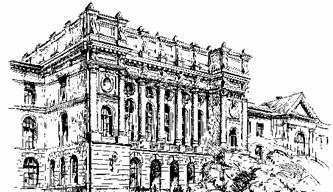
\includegraphics[scale=0.7]{../pics/spbpu.jpg}\\[2cm]
		
		\huge Реферат по компьютерной алгебре\\[0.5cm] % название работы, затем отступ 0,5см
		\huge Алгоритмы сжатия изображений\\[3cm]

	\end{center}	
	
	\begin{flushright} % выравнивание по правому краю
		\begin{minipage}{0.25\textwidth} % врезка в половину ширины текста
			\begin{flushleft} % выровнять её содержимое по левому краю

				\large\textbf{Студенты:}\\
				\large В.В. ~Дьячков\\
				\large А.А. ~Жуйков\\
				\large А.Ю. ~Ламтев\\
				\large Ю.И. ~Леженин\\
				\large {Группа:} 13501/4\\
				
				\large \textbf{Преподаватель:}\\
				\large И.А. ~Малышев\\

			\end{flushleft}
		\end{minipage}
	\end{flushright}
	
	\vfill % заполнить всё доступное ниже пространство

	\begin{center}
	\large Санкт-Петербург\\
	\large \the\year % вывести дату
	\end{center} % закончить выравнивание по центру
\thispagestyle{empty} % не нумеровать страницу
\end{titlepage} % конец титульной страницы

\vfill % заполнить всё доступное ниже пространство
